%% LyX 2.0.6 created this file.  For more info, see http://www.lyx.org/.
%% Do not edit unless you really know what you are doing.
\documentclass{standalone}
\usepackage{graphicx}

\makeatletter

%%%%%%%%%%%%%%%%%%%%%%%%%%%%%% LyX specific LaTeX commands.
%% A simple dot to overcome graphicx limitations
\newcommand{\lyxdot}{.}


\makeatother

\begin{document}
\begin{wrapfigure}{r}[0.1\columnwidth]{0.6\columnwidth}% 
\vspace{-40pt}\hspace{-1cm}
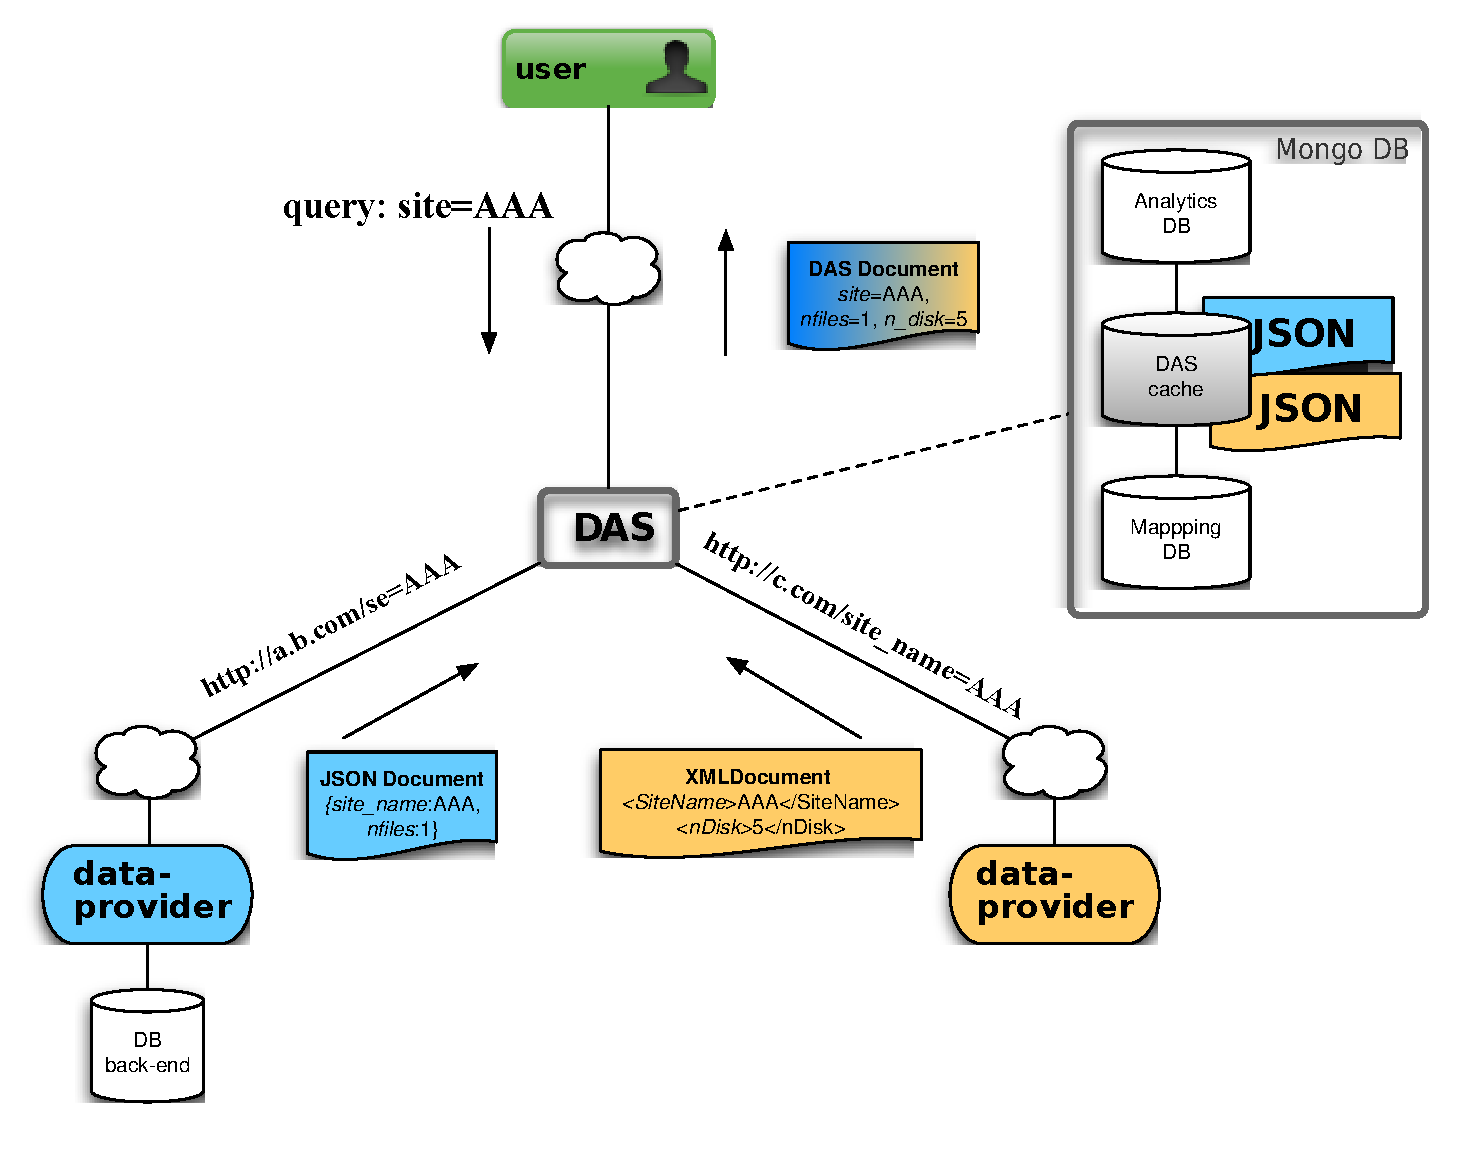
\includegraphics[width=0.55\columnwidth]{images/das}
\vspace{-2.5cm}
\caption{DAS workflow}
\vspace{-4cm}
\end{wrapfigure}% 

\textbf{''CMS Data Aggregation System'' (DAS):}
\begin{itemize}
\item accepts simple structured queries
\item integrates heterogeneous services

\begin{itemize}
\item parse the query \& contact services
\item eliminate inconsistencies in responses:

\begin{itemize}
\item entity naming
\item data formats {\footnotesize{(XML, JSON)}}{\footnotesize \par}
\end{itemize}
\item combine them
\end{itemize}
\item requires only minimal service mappings

\begin{itemize}
\item no predefined schema
\item minimal effort in defining services
\end{itemize}
\end{itemize}

\paragraph{Queries}

must specify: entity to be retrieved and filtering criteria. Optionally,
the results can be further filtered, sorted or aggregated

\includegraphics[width=1\textwidth]{/home/vidma/DAS_paper/figures/DASQL_structure}
\end{document}
